\documentclass[fontset=none]{ctexart}

\usepackage[T1]{fontenc}
\usepackage{fontspec}
\setCJKmainfont{SimSun}
% Latin Modern
\renewcommand*\ttdefault{txtt} % 改等宽字体

\setcounter{tocdepth}{5}
\setcounter{secnumdepth}{5}
% -1 part
% 0 chapter
% 1 section
% 2 subsection
% 3 subsubsection
% 4 paragraph
% 5 subparagraph

\usepackage{cite}
\usepackage{geometry}
\geometry{a4paper,scale=0.8}

\usepackage{algorithm}  
\usepackage{algorithmicx}  
\usepackage{algpseudocode}
\makeatletter
\newenvironment{breakablealgorithm}
  {% \begin{breakablealgorithm}
   \begin{center}
     \refstepcounter{algorithm}% New algorithm
     \hrule height.8pt depth0pt \kern2pt% \@fs@pre for \@fs@ruled
     \renewcommand{\caption}[2][\relax]{% Make a new \caption
       {\raggedright\textbf{\ALG@name~\thealgorithm} ##2\par}%
       \ifx\relax##1\relax % #1 is \relax
         \addcontentsline{loa}{algorithm}{\protect\numberline{\thealgorithm}##2}%
       \else % #1 is not \relax
         \addcontentsline{loa}{algorithm}{\protect\numberline{\thealgorithm}##1}%
       \fi
       \kern2pt\hrule\kern2pt
     }
  }{% \end{breakablealgorithm}
     \kern2pt\hrule\relax% \@fs@post for \@fs@ruled
   \end{center}
  }
\makeatother

\usepackage{amsmath}
\usepackage{amssymb}
\usepackage{graphicx}
\usepackage{subfigure}
\usepackage{changepage}
\usepackage{multirow}
\usepackage{url}

\usepackage{amsthm}
\newtheorem{theorem}{Theorem}[section]
\newtheorem{lemma}[theorem]{Lemma}
\newtheorem{proposition}[theorem]{Proposition}
\newtheorem{corollary}[theorem]{Corollary}
% \newtheorem{remark}{Remark}[section]
\newtheorem{example}{Example}[section]
\newenvironment{solution}{\begin{proof}[Solution]}{\end{proof}}
\theoremstyle{definition}
\newtheorem{definition}{Definition}[section]
\theoremstyle{remark}
\newtheorem*{remark}{Remark}

\usepackage[colorlinks, linkcolor=black, citecolor=blue, bookmarksnumbered]{hyperref}
% \hypersetup{
% 	colorlinks=true,
% 	linkcolor=cyan,
% 	filecolor=blue,      
% 	urlcolor=red,
% 	citecolor=green,
% }

\usepackage{fancyhdr}
\pagestyle{fancy}
\renewcommand{\sectionmark}[1]{\markright{\thesection\ #1}}
\fancyhf{}
\cfoot{\thepage}
\lhead{\rightmark}
% \rightmark 当前的节名
% \leftmark 当前的章名
% \(l/c/r)head{}, \(l/c/r)foot{}
\renewcommand{\headrulewidth}{0.4pt}
\renewcommand{\footrulewidth}{0pt}

\renewcommand\refname{References}
\renewcommand\contentsname{Contents}
\renewcommand\figurename{Figure}

\begin{document}

\begin{titlepage}
    \begin{center}
        \vspace*{1cm}
            
        \Huge
        \textbf{Traffic Network Flow\\ Estimation Based On\\ Social Network Influence Model}
            
        \vspace{0.5cm}
        \LARGE
        First Report\\
            
        \vspace{1.5cm}
            
        \textbf{11812804}  董\quad 正\\
        \textbf{11810419}  王焕辰\\
        \textbf{11811305}  崔俞崧\\

        \vspace{0.5cm}
        Supervisior: 宋轩
            
        \vfill
            
        
\includegraphics[width=\textwidth]{images/sustc.png}
            
        \vspace{0.2cm}
            
        \Large
        Department of Computer Science and Engineering\\
        \vspace{0.5cm}
        Oct. 2021
            
    \end{center}
\end{titlepage}

\tableofcontents

\clearpage
\section{Preliminaries}
\subsection{Introduction}
In this semester, we will try to build a traffic flow estimation system based on graph neural network and
social network influence model. Breifly, the structure of the whole system is

\begin{figure}[htb]
  \centering
  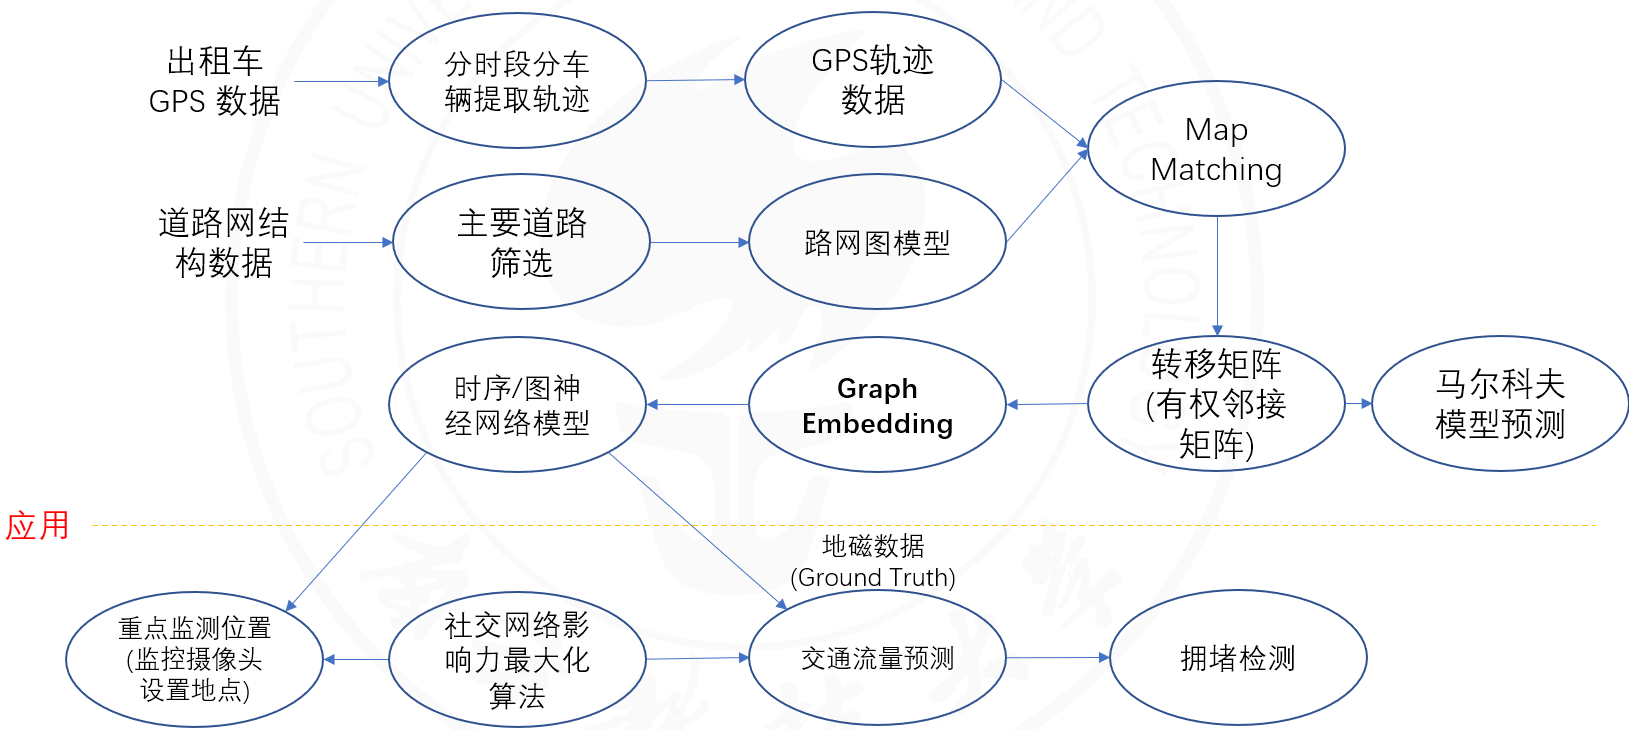
\includegraphics[width=\textwidth]{images/7-1-1.png}
  \caption{System Structure}
  \label{fig: structure}
\end{figure}

\begin{enumerate}
  \item Process taxi GPS data to get tracks
  \item Process road network data to get a basic graph model
  \item Match tracks to each road and get the adjacent matrix of the graph
  \item Try a simple prediction based on Markov model
  \item Graph embedding (the most important part)
  \item Build a neural network model for prediction
  \item Combine social network influence algorithms to predict traffic network flow, use geomagnetic data as one of the ground truth
  \item Applications: traffic surveillance camera position and traffic jam detection
\end{enumerate}

\subsection{Report Contents}
Breifly, we will state our work in this report as
\begin{itemize}
  \item Taxi Data Processing by 崔俞崧
  \item Geomagnetic Data Processing by 王焕辰
  \item Road Graph Model \& Map Matching by 董正
\end{itemize}

\clearpage
\section{Taxi Data Processing}
\subsection{Dataset}
\begin{itemize}
  \item Data source: Shenzhen Municipal Government 
  \item Region: Shenzhen
  \item Time: 2019-12-01 to 2019-12-13
  \item Content: Taxi vehicle trajectory data
    \begin{itemize}
      \item License number
      \item Longitude and latitude
      \item Speed
      \item License type
    \end{itemize}
\end{itemize}

\begin{figure}[htb]
  \centering
  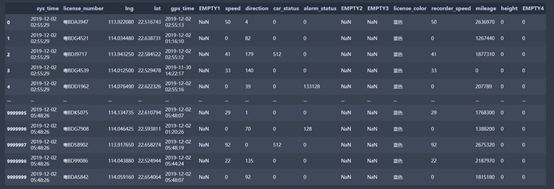
\includegraphics[width=\textwidth]{images/7-2-1.png}
  \caption{Dataset}
  \label{fig: 721}
\end{figure}

\subsection{Data Processing}
Because trajectory data are unprocessed original data, there are error data in the process of data acquisition, in addition, the format of original data does not meet our requirements, so the data need to be screened to a certain extent.
\begin{enumerate}
  \item Sort by GPS time and remove duplicate data of the records.
  \item Remove data with the wrong date. There is data loss when recording, and there are many data records outside the specified date range that need to be filtered.
  \item Remove the records of speed 0 and speed record too large (>120km/h). The records we needed is the track information generated when the vehicle is running instead of when the vehicle is standing still. The record with the speed 0 has no impact on the track. And the record with excessive speed is obviously the error data. These data need to be removed.
  \item Delete the records that cannot be matched with the road segment in the matching process. What is needed in processing is the traffic flow information on each road section, and the records that cannot match with the road section have no use significance.
\end{enumerate}

\subsection{Data Visualization}
Statistics the speed distribution and draw the speed distribution figure. Then processing the speed data using the statistics result.

We can see that there are vast number of 0 speed records and some records with speed over 150 km/h. These records need to be processed to meet the demand.

\begin{figure}[htb]
  \centering
  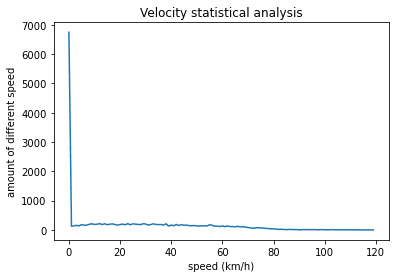
\includegraphics[width=0.8\textwidth]{images/7-2-2.png}
  \caption{The original speed distribution}
  \label{fig: 722}
\end{figure}

\clearpage
After processing, the distribution of speed records are very close to reality. Most of the vehicles records are in urban areas so the speed is not very large, while a small number of vehicles records are on expressways where the speed value is relatively high (about 80 km/h).

\begin{figure}[htb]
  \centering
  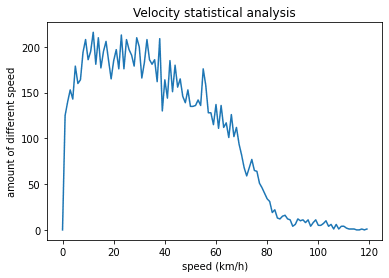
\includegraphics[width=0.8\textwidth]{images/7-2-3.png}
  \caption{Speed distribution after process}
  \label{fig: 723}
\end{figure}

\clearpage
Visualize the all-day trajectory of a vehicle, the results can be obtained as shown in the figure below
(Classify taxi tracks according to different orders through GPS time, so as to better distinguish different tracks)
\begin{figure}[htb]
  \centering
  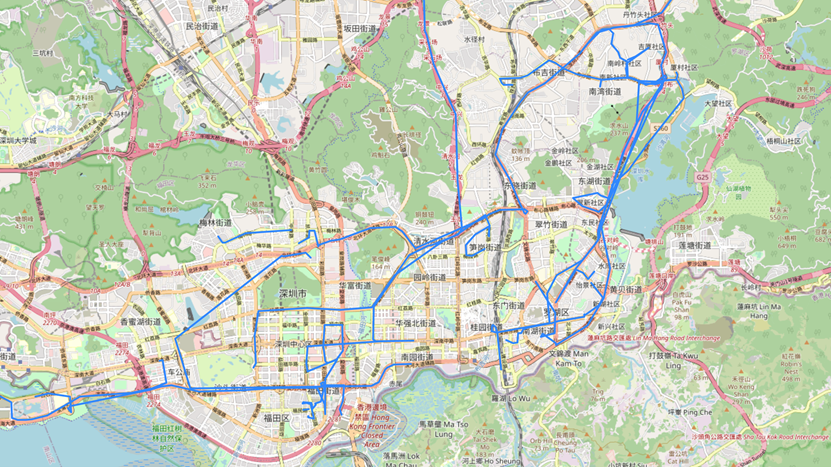
\includegraphics[width=0.8\textwidth]{images/7-2-4.png}
  \label{fig: 724}
\end{figure}
\begin{figure}[htb]
  \centering
  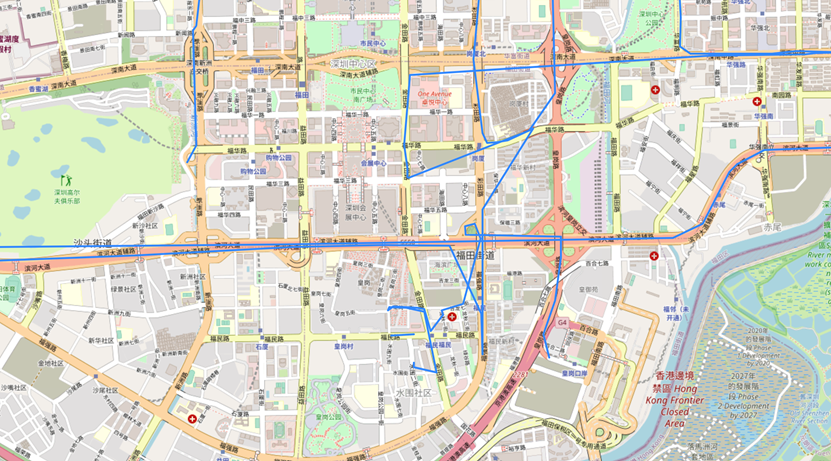
\includegraphics[width=0.8\textwidth]{images/7-2-5.png}
  \label{fig: 725}
\end{figure}

\clearpage
\section{Geomagnetic Data Processing}
\subsection{Dataset}
\begin{itemize}
  \item Data source: Communications Bureau of Shenzhen 
  \item Region: Shenzhen
  \item Time: 2019-12-02
  \item Content: Traffic flow data of main roads in Shenzhen
    \begin{itemize}
      \item Cross id
      \item Upload time
      \item Speed
      \item Car type
      \item \dots
    \end{itemize}
\end{itemize}
\begin{figure}[htb]
  \centering
  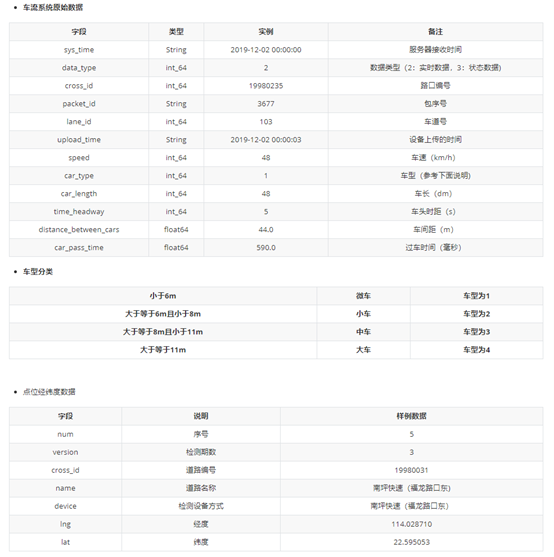
\includegraphics[width=0.8\textwidth]{images/7-3-1.png}
  \label{fig: 731}
\end{figure}

\subsection{Data Processing}
Because traffic flow data from geomagnetic device is unprocessed original data, there is error data in the process of data acquisition, especially the time data. Besides, there are many kinds of device not only geomagnetic sensor and there are also 2 kinds of data type. Only use data detected by geomagnetic and real time data, so the data need to be screened to a certain extent. In addition, Visualizing the distribution of each point on the road network map in Shenzhen to detect the drift of geomagnetic position information.
\begin{enumerate}
  \item Extract the data whose data type is 2 and device is geomagnetic sensor.
  \item Remove duplicate data of the records.
  \item Remove data with the wrong date. There is data loss when recording, and there are many data records outside the specified date range, such as 239:69:123, which need to be filtered.
\end{enumerate}
\begin{figure}[htb]
  \centering
  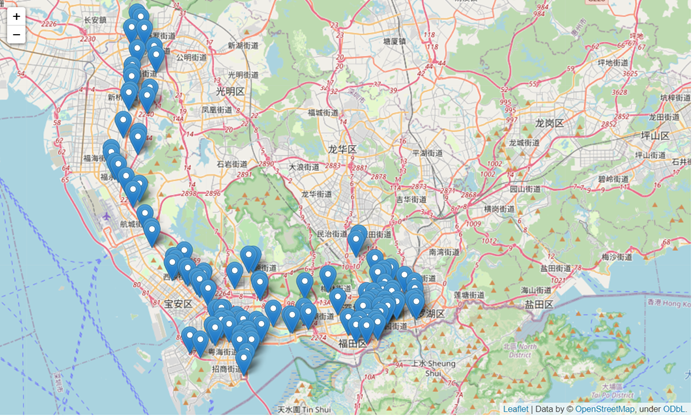
\includegraphics[width=\textwidth]{images/7-3-2.png}
  \label{fig: 732}
  \caption{Distribution of Each Point}
\end{figure}

\subsection{Data Visualization}
Group traffic flow data by 15 min as time interval and draw line charts of the speed and traffic flow over time to verify the authenticity.
\clearpage
\begin{figure}[t]
  \centering
  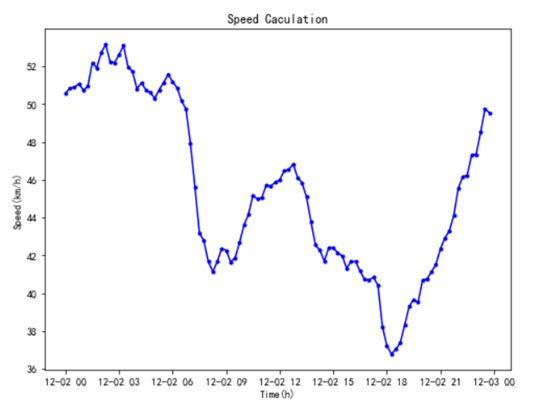
\includegraphics[width=0.8\textwidth]{images/7-3-3.png}
  \caption{Mean Speed over Time}
  \label{fig: 733}
\end{figure}
\begin{figure}[b]
  \centering
  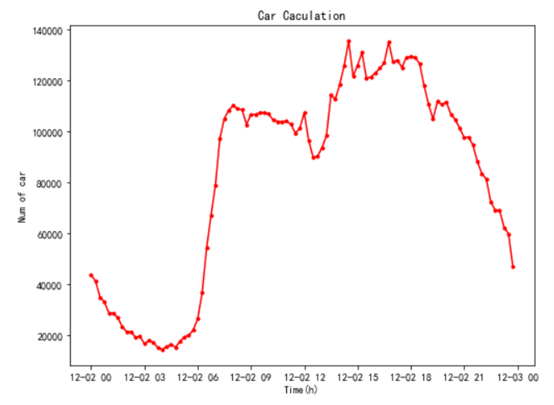
\includegraphics[width=0.8\textwidth]{images/7-3-4.png}
  \caption{Mean Traffic flow over Time}
  \label{fig: 734}
\end{figure}

\clearpage
Visualize 10 main roads to the neighborhood in speed and traffic flow grid charts during heavy traffic hours to reflect road congestion and its spread, it can also verify whether it conforms to the real situation of main road and analyze the outliers to find out the reasons or remove them.
\begin{figure}[h!]
  \centering
  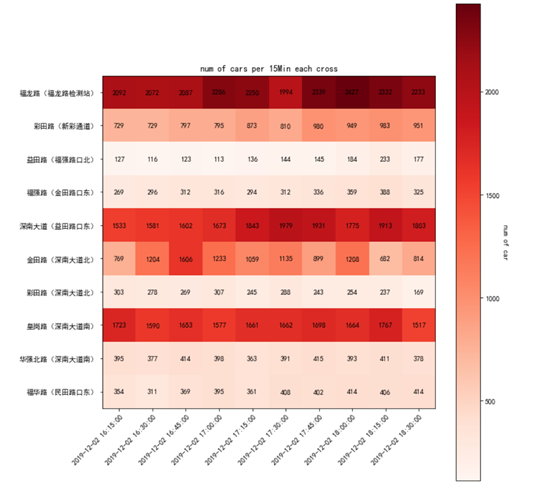
\includegraphics[width=0.6\textwidth]{images/7-3-5.png}
  \caption{Traffic Flow Grid Chart}
  \label{fig: 735}
\end{figure}
\begin{figure}[h!]
  \centering
  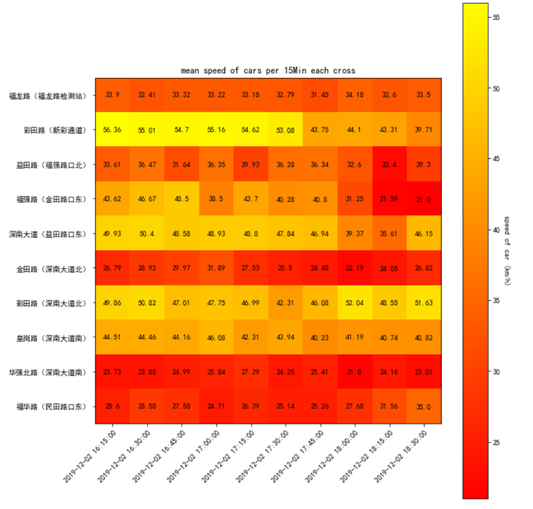
\includegraphics[height=\dimexpr\pagegoal-\pagetotal-4\baselineskip\relax,
                  width=0.6\textwidth,
                  keepaspectratio]
                  {images/7-3-6.png}
  \caption{Speed Grid Chart}
  \label{fig: 736}
\end{figure}

According to the geomagnetic data of a day, the traffic flow of each road in each time period is counted and divided into groups by roads at intervals of 15 minutes. Circle, corresponding radius of traffic flow, Selenium library and Image library are used to synthesize the dynamic traffic flow map.
\begin{figure}[htb]
  \centering
  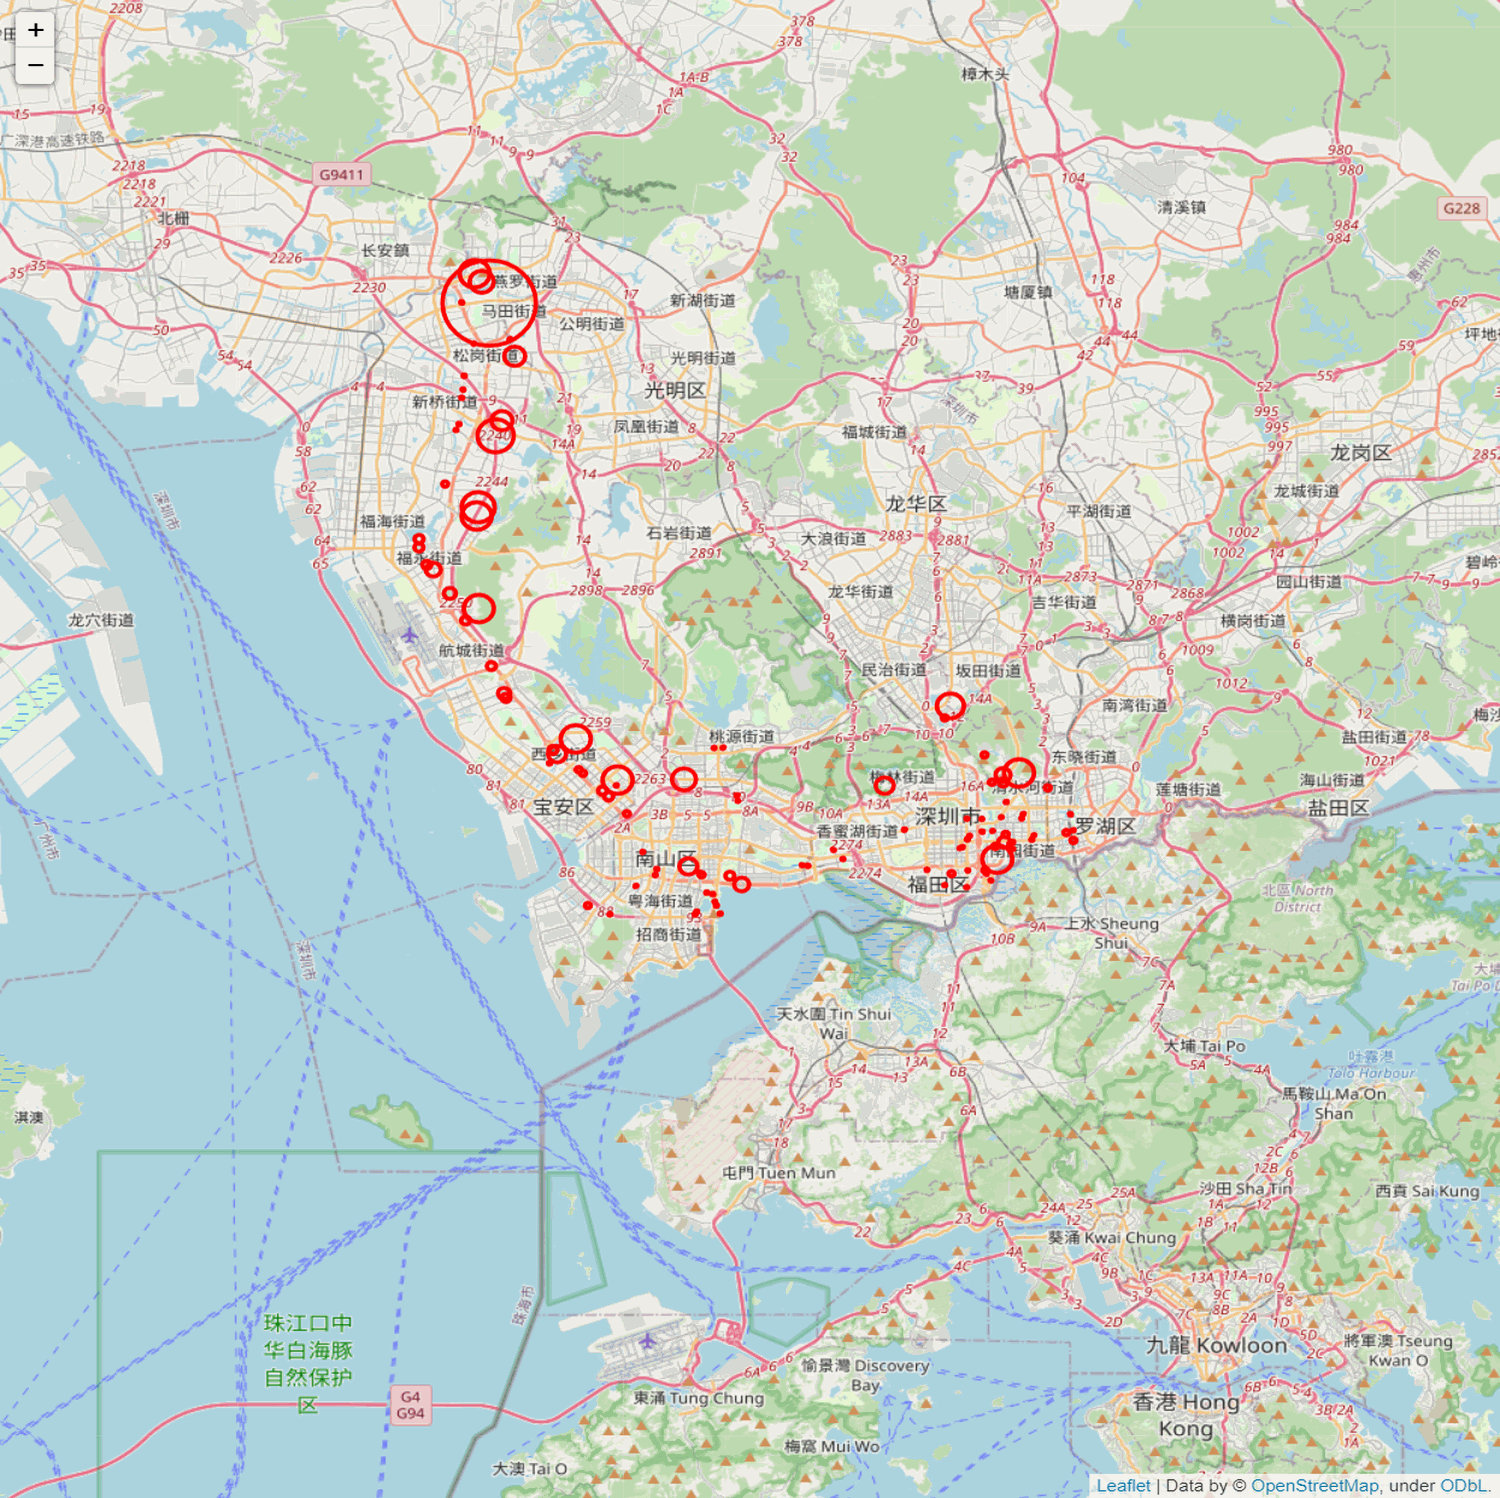
\includegraphics[width=\textwidth]{images/7-3-7/f5ef9dc31d044acac988911ed92b0494EgYhqvGPburiSExo-22.png}
  \caption{Dynamic Traffic Flow Map}
  \label{fig: 737}
\end{figure}

\clearpage
\section{Road Graph Model \& Map Matching}
\subsection{Road Network}
Use \texttt{osmnx} library of \textit{Python} to get the road network graph of Shenzhen.
In addition, specify the type as ``drive'' in order not to get pedestrians and so on.

\begin{figure}[htb]
  \centering
  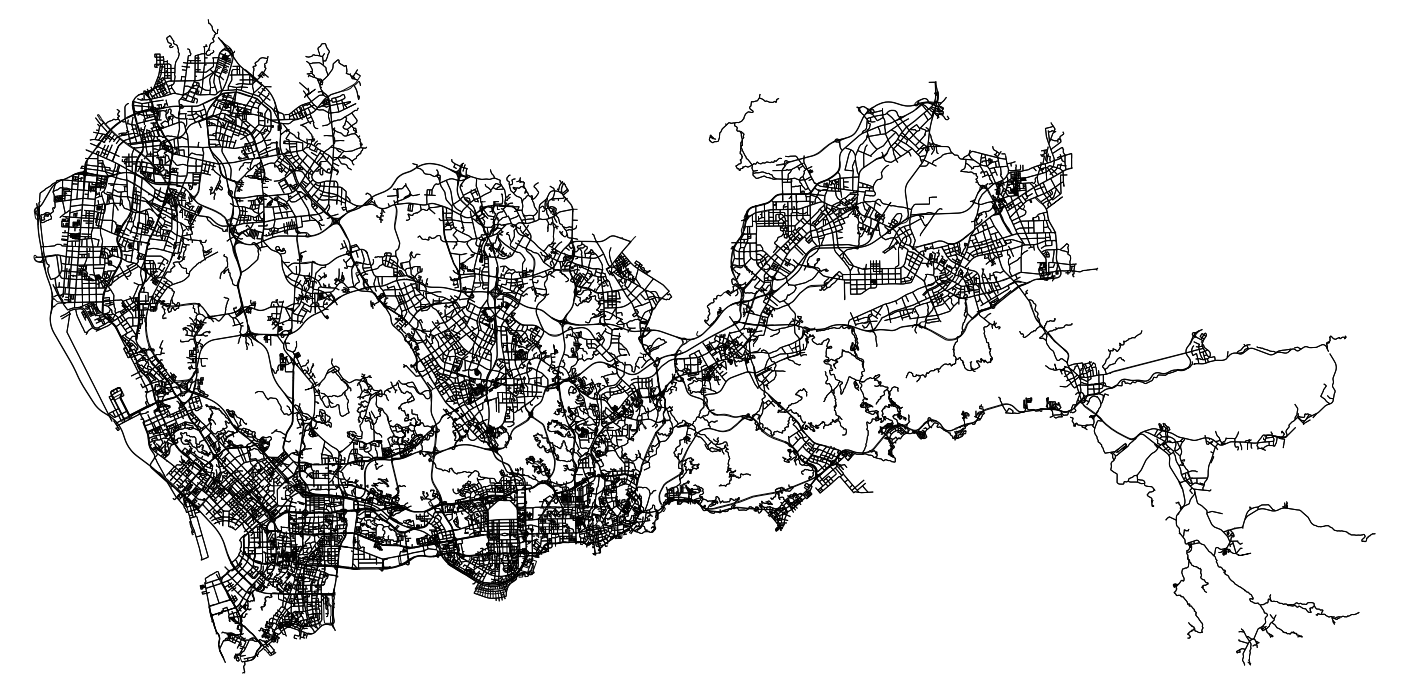
\includegraphics[width=\textwidth]{images/7-4-1.png}
  \caption{Road Network}
  \label{fig: rn}
\end{figure}

In this graph, node represents the point of intersection of roads. And edge represents road, whose
weight contains the geometry information of the road. However, in our model, we want to set roads as nodes,
and edges only represent connectivity. Use \texttt{networkx.line\_graph()} to transform.

\clearpage
The network is still very complex. Therefore, the next step is to choose main roads to simplify the network.
In edge weight, we find there is an attribute called \texttt{highway}. According to the document of \textit{OpenStreetMap},
we chose some of the types as the major, and filtered all the roads.

\begin{figure}[htb]
  \centering
  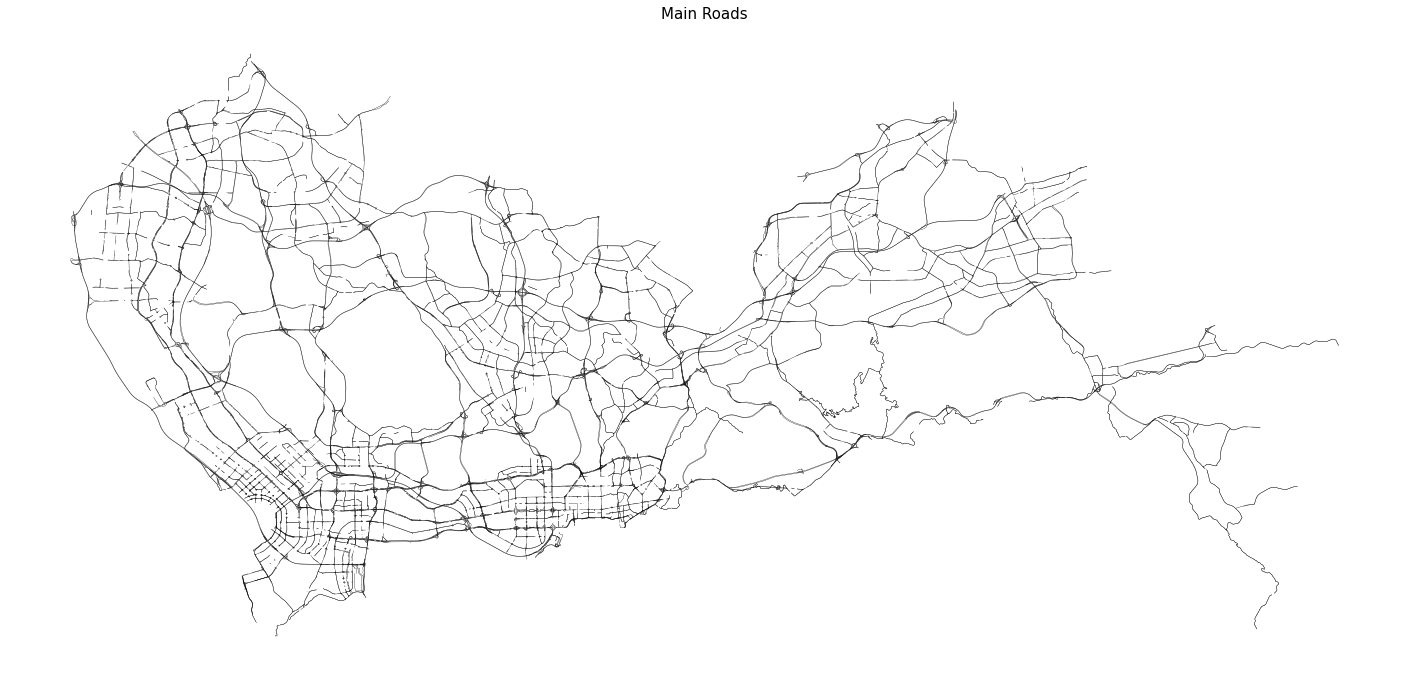
\includegraphics[width=\textwidth]{images/7-4-2.png}
  \caption{Main Road Network}
  \label{fig: mrn}
\end{figure}

\subsection{Map Matching}
In our dataset, a road is represented as a line, however, it should be an area in real world.
Besides, it is hard to match a point to a 2-D line. Therefore, we need to convert a road to an area in advance.

Use method \texttt{buffer()} in \textit{shapely} package.
\begin{figure}[htb]
  \centering
  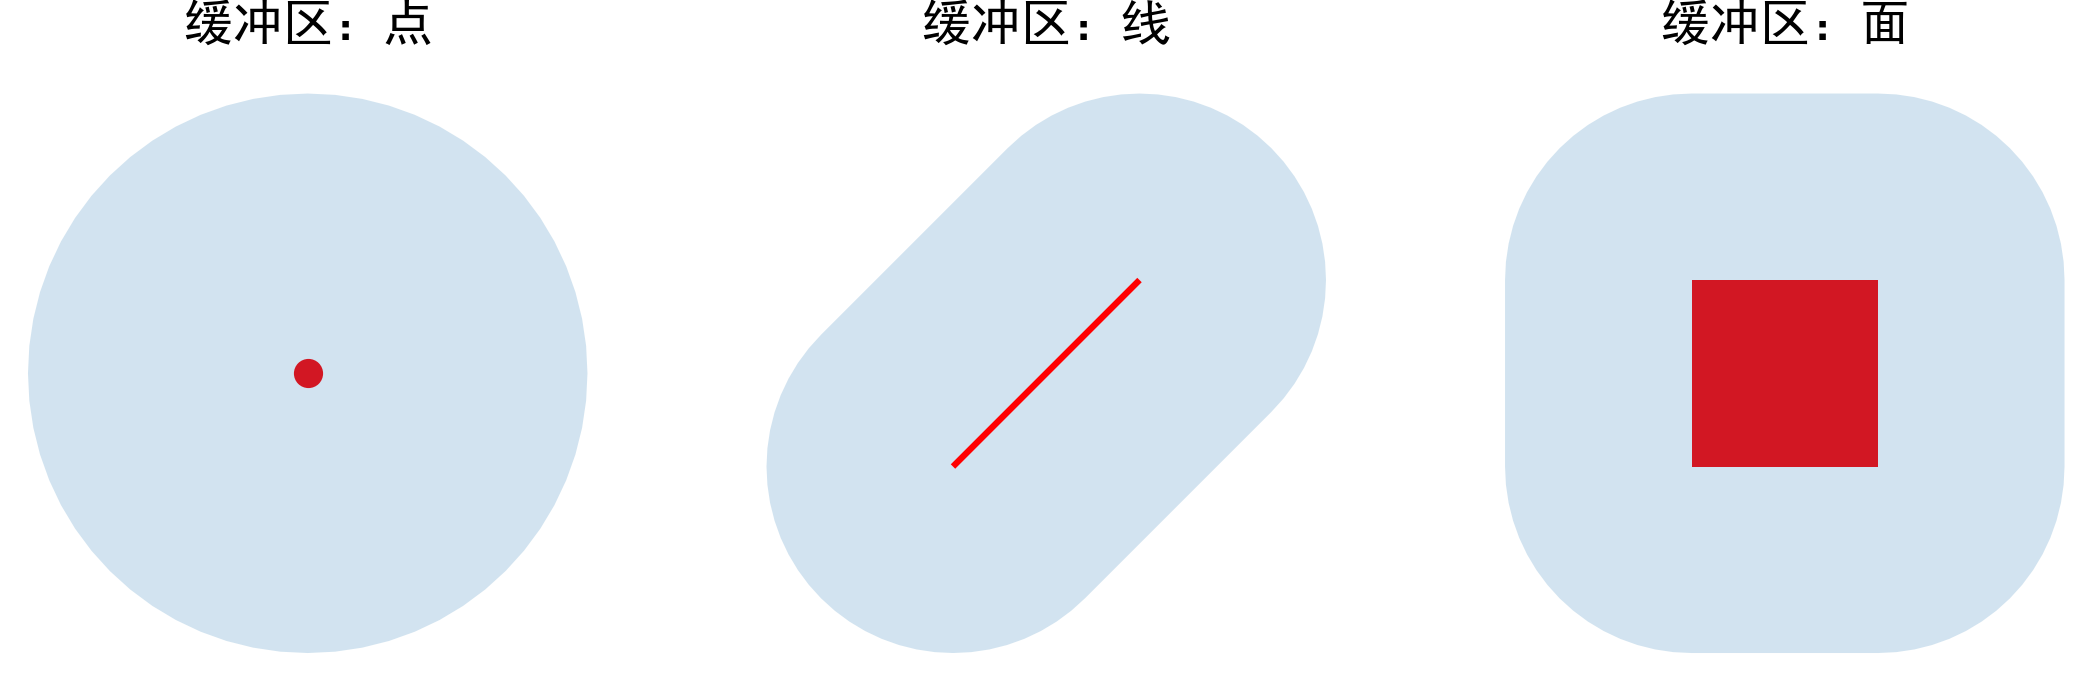
\includegraphics[width=0.9\textwidth]{images/buffer_example.png}
  \caption{\texttt{buffer()}}
  \label{fig: buffer}
\end{figure}

The \texttt{buffer()} method will convert a \texttt{Line} to a \texttt{Polygon}.

After that, we take the advantage of the continuity of tracks to do map-matching.
\begin{enumerate}
  \item Rename the id of every remaining road
  \item Initialize transition matrix
  \item Downsample the track, delete the points which are very close in time (<30s)
  \item Find the center of every road
  \item Find the median of the track
  \item Sort all the roads according to the distance between the center and the median
  \item For each GPS point, use \texttt{contains()} function to match it to a road
  \item Modify transition matrix
\end{enumerate}

The expected time complexity is about $O(n^2\log n+Cn^2)$.

Finally the output is a weighted adjacent matrix (transition matrix), which is the true representaion of the graph.

After that, we can do a simple statistical prediction.

What's more,
\begin{itemize}
  \item Split tracks to different time intervals to increase the accuracy of prediction
  \item Use multiple processers to accelerate
\end{itemize}


% \clearpage
% \phantomsection
% \addcontentsline{toc}{section}{References}
% \bibliographystyle{ieeetr}
% \bibliography{references}

\end{document}